\label{sec:intro}

\subsection{Oscillators}
Oscillators can be described as a repetitive motion of some measure about a central value which is often the point of equilibrium. This term is often used in mechanical systems but it must also be noted that oscillations occur in dynamic systems too, such as economic graphs, geothermal temperatures across areas and periodic ``firing'' of fireflies in nature. Some examples of oscilating objects can be found in Figure~\ref{fig:intro_samples}. 

\begin{figure}[h]
\centering
\begin{subfigure}{.4\textwidth}
  \centering
  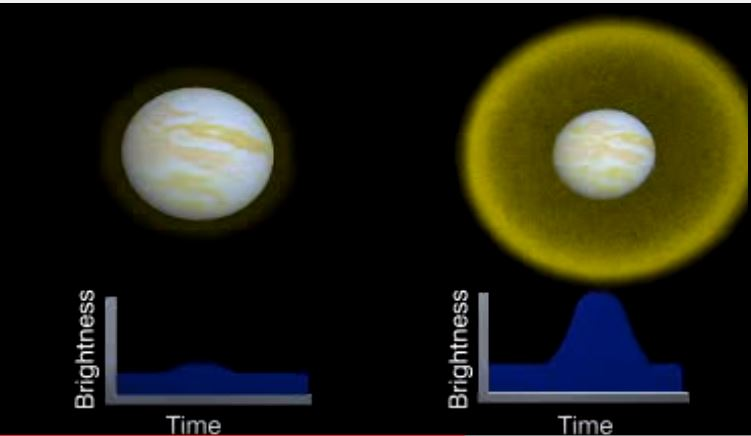
\includegraphics[width=\textwidth]{imgs/cepheid}
  \caption{Cepheid Stars that are known to flash occasionally. Such a flash is an example of an oscilation. }
\end{subfigure}%
\space\space\space
\begin{subfigure}{.5\textwidth}
  \centering
  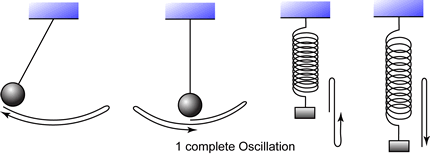
\includegraphics[width=\textwidth]{imgs/oscillation}
  \caption{An pendulum swinging to the left and right and a spring oscilating up and down. }
\end{subfigure}
\caption{Some examples of oscilating objects}
\label{fig:intro_samples}
\end{figure}


\subsection{Coupling}
Coupled Oscillation are a slightly more complex form of ordinary oscillators. In this model the oscillators are connected such that energy can be transferred between them. This motion can be very complex and does not have to be periodic. However, in the bigger scheme of things, every oscillator can be viewed as having a very well defined frequency of its own. Perhaps the simplest example of coupling could is a gear that transmits torque between two shafts (see Figure~\ref{fig:intro_gear}) that are not collinear. 

\begin{figure}[h]
  \centering
  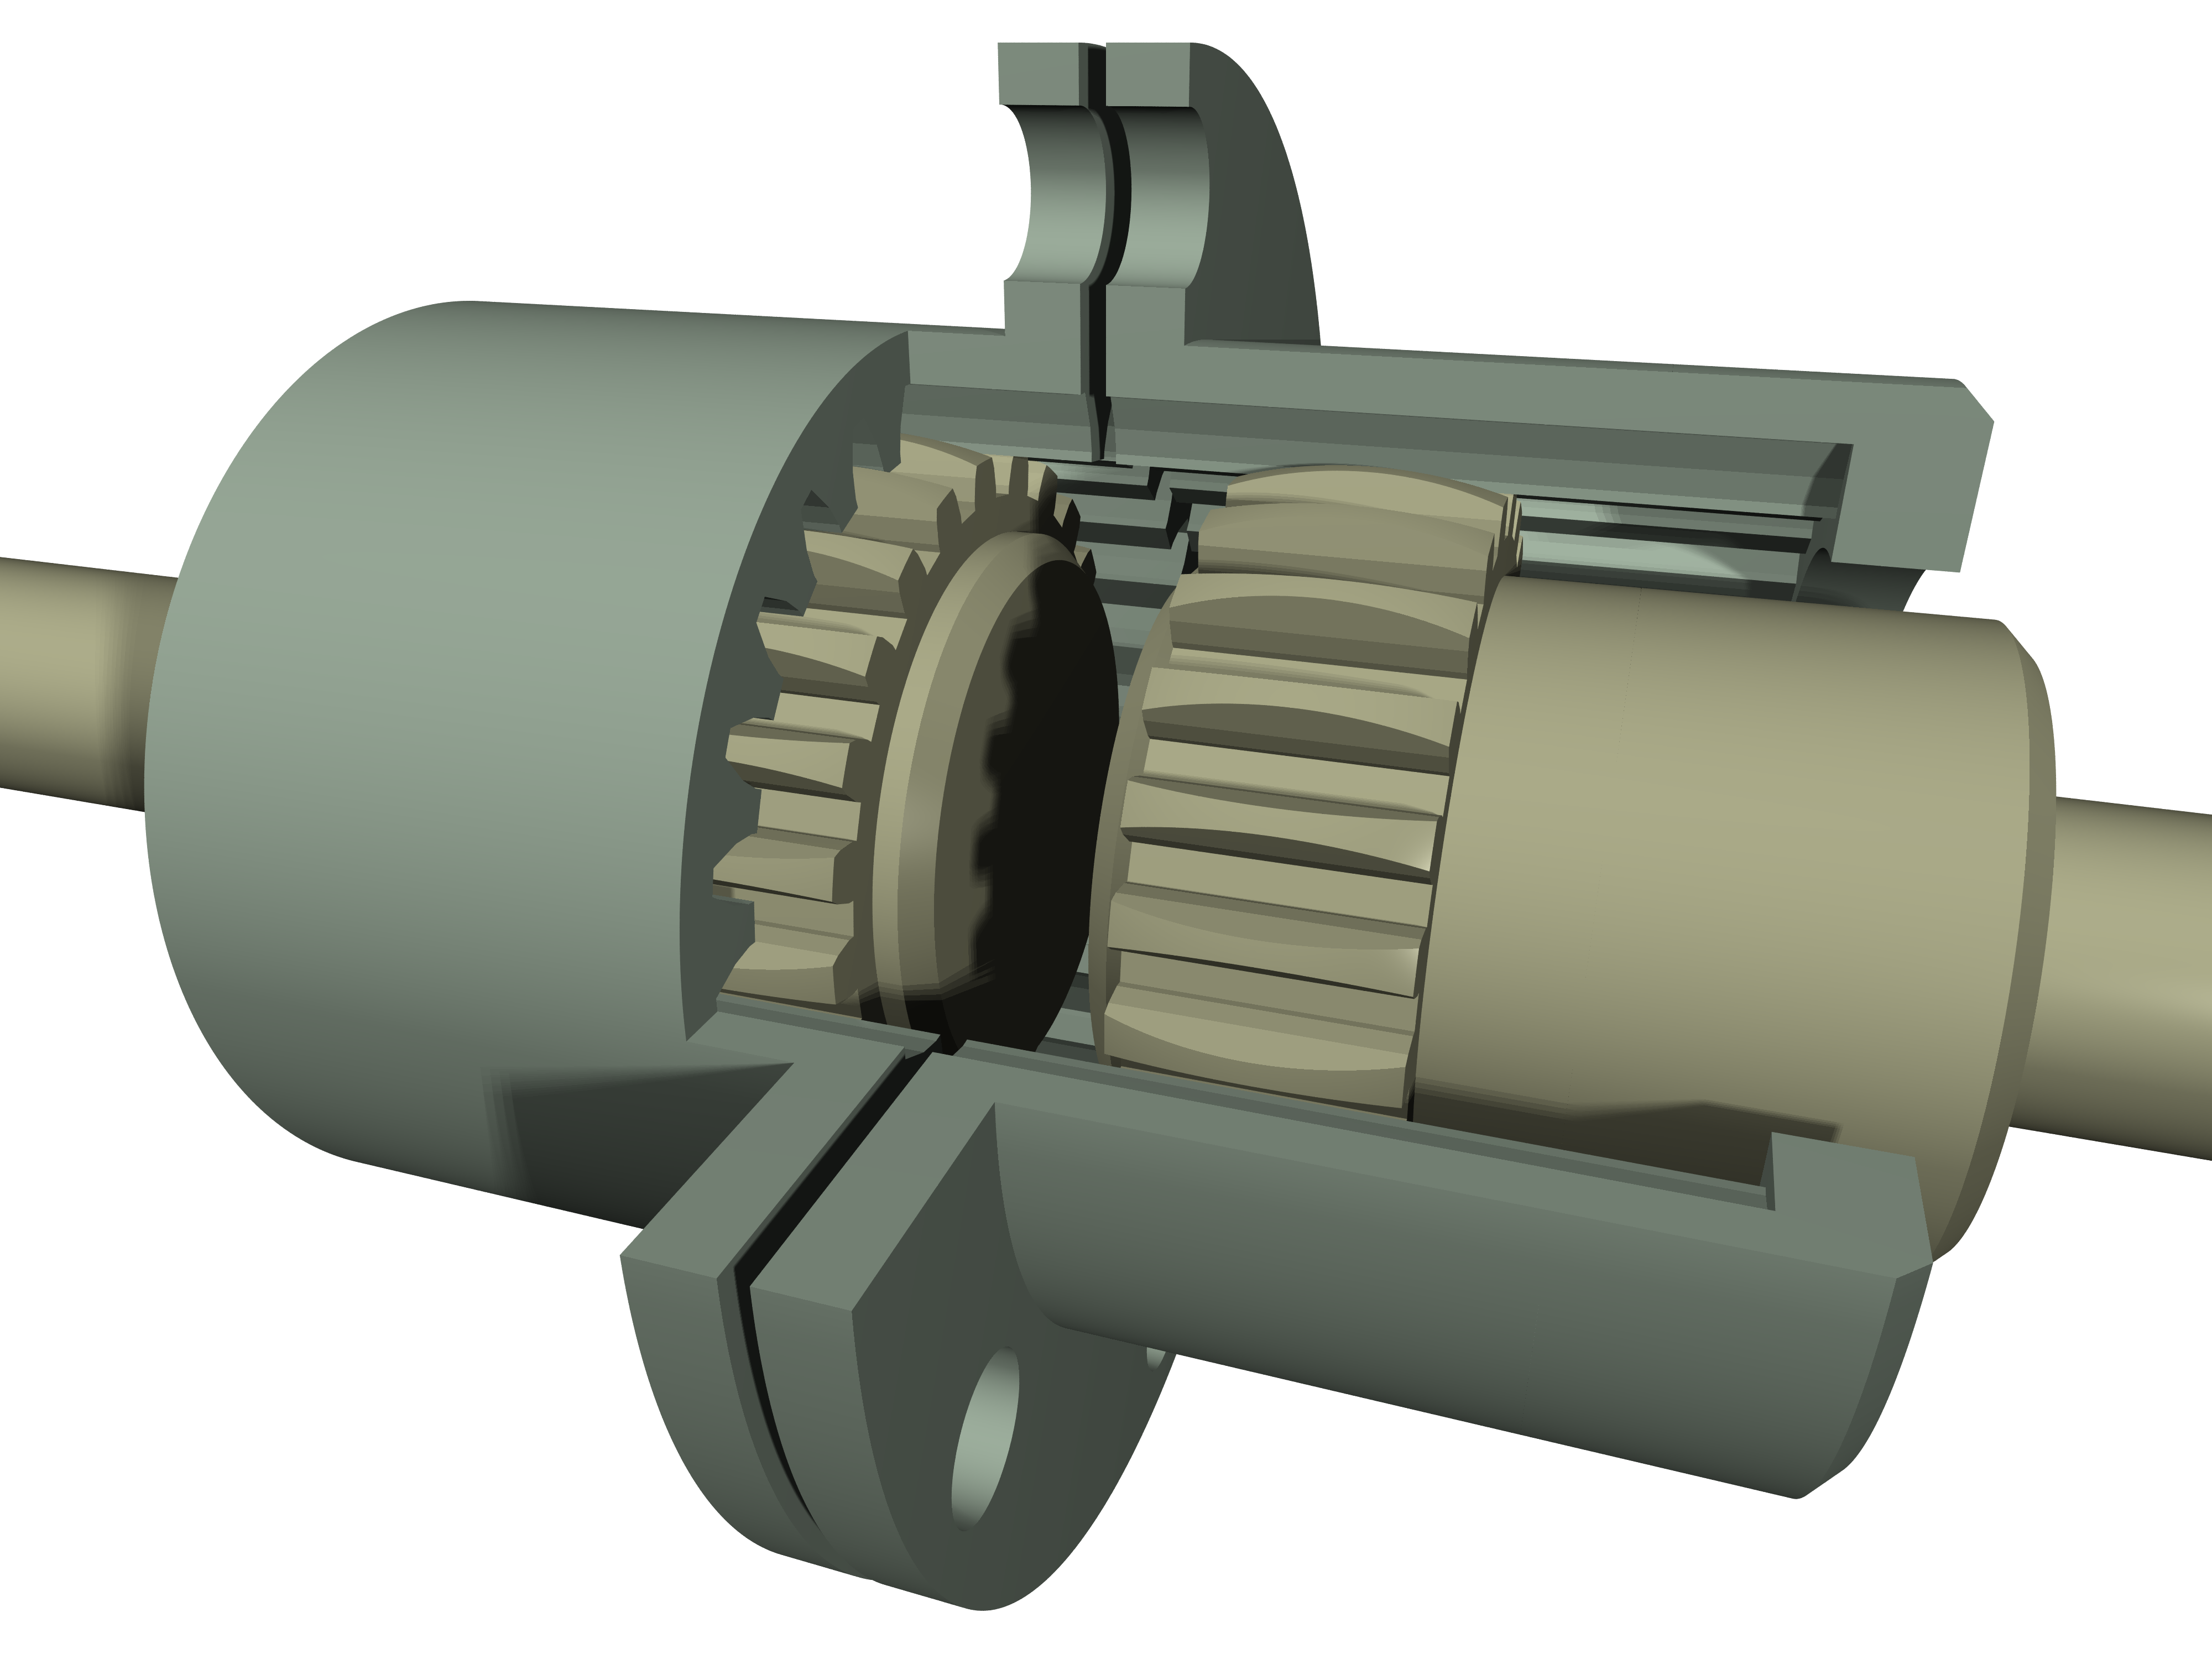
\includegraphics[width=.5\textwidth]{imgs/gear}
  \caption{Image of a gear that transmits torque beween two non-collinear shafts. }
  \label{fig:intro_gear}
\end{figure}

A slightly more complex situation arises when two pendulums are joined together by an energy medium, for example a string. As we can see in Figure~\ref{fig:intro_couple}, the two pendula have opposite amplitudes: The first pendulum only attains its maximum amplitude when the second has its lowest one. This form of synchronization behaviour can only be achieved after sufficient time has passed. 

\begin{figure}[h]
\centering
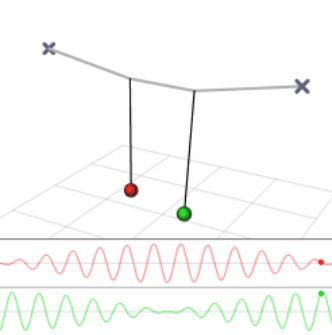
\includegraphics[width=.5\textwidth]{imgs/couple}
\caption{Two oscilating springs that exhibit coupling behaviour because they are connected through a string}
\label{fig:intro_couple}
\end{figure}

\subsection{Attaining Synchronisation}

In any oscilating system of multiple objects synchronization can occur in two ways, (1) through coupling or (2) through randomness. In the first case some form of communication between the oscilators occurs allowing them to couple. In the second case it just so happens that they start out in a similar situation and are naturally synchronized. In this study we are only interested in the first case. 

Communication can be achieved by using a medium such as a string between oscilators or by just the intrinsic tendency of natural beings to produce a unison of movement, such as fireflies flashing or humans clapping in a room. 

\subsection{The Firefly model}

The firefly flashing, more commonly known as the firefly model, is a classic example of synchronisation. This is modelled in detail by Kuramoto oscilators which is the main topic of study for this report. We will introduce these in the next section. 

\begin{figure}[h]
	\centering
	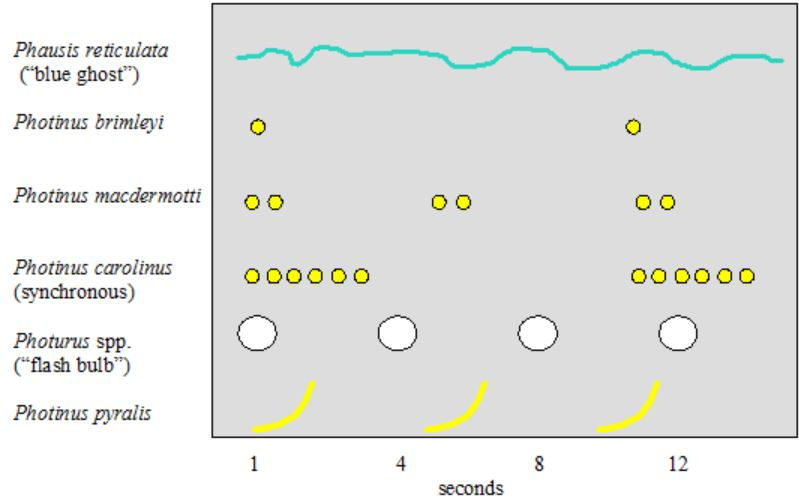
\includegraphics[width=\textwidth]{imgs/flash}
	\caption{Behaviour of fireflies flashing over the time. }
	\label{fig:intro_flash}
\end{figure}
 
The light patterns of fireflies are part of a mating display that the male fireflies use to attract the female ones. If successful, the female replies back with a characteristic flash of it own. Although this is synchronisation on its own, there are a few species of fireflies where more than 2 individuals can synchronize. These species are usually observed in large groups, all flashing together in unison.

As we can see in Figure~\ref{fig:intro_flash}, all of the species fire of one after another in a synchronized fashion except the blue one which seems to be random. 

\subsection{Goal}
Our goal for this study is to investigate Kuramoto oscilators with negative coupling co-efficients. We will define what exactly a coupling coefficient is and what negative coefficients mean in the next section, but one can intuitively think of it as a number measuring the strength of attraction between two oscilators. 
The reason we specifically want to use negative coupling coefficients is because, in contrast to positive coefficients, it is much easier to generate complex synchronisation patterns. We want to study and observe these patterns and investigate if we can construct systems that generate desired patterns. 

In Section~\ref{sec:kuramoto} we will introduce the Kuramoto oscillator, explain its equations, some required background knowledge as well as our implementation of it. In Section~\ref{sec:negative} we continue with describing the patterns we encountered when using negative coefficients. We then move on to describe a method which can be used to re-create arbitrary patterns in Section~\ref{sec:patterns} before concluding in Section~\ref{sec:conclusion}. 